\documentclass[]{article}
\usepackage{lmodern}
\usepackage{amssymb,amsmath}
\usepackage{ifxetex,ifluatex}
\usepackage{fixltx2e} % provides \textsubscript
\ifnum 0\ifxetex 1\fi\ifluatex 1\fi=0 % if pdftex
  \usepackage[T1]{fontenc}
  \usepackage[utf8]{inputenc}
\else % if luatex or xelatex
  \ifxetex
    \usepackage{mathspec}
  \else
    \usepackage{fontspec}
  \fi
  \defaultfontfeatures{Ligatures=TeX,Scale=MatchLowercase}
\fi
% use upquote if available, for straight quotes in verbatim environments
\IfFileExists{upquote.sty}{\usepackage{upquote}}{}
% use microtype if available
\IfFileExists{microtype.sty}{%
\usepackage{microtype}
\UseMicrotypeSet[protrusion]{basicmath} % disable protrusion for tt fonts
}{}
\usepackage[margin=1in]{geometry}
\usepackage{hyperref}
\hypersetup{unicode=true,
            pdftitle={Chocolate},
            pdfborder={0 0 0},
            breaklinks=true}
\urlstyle{same}  % don't use monospace font for urls
\usepackage{color}
\usepackage{fancyvrb}
\newcommand{\VerbBar}{|}
\newcommand{\VERB}{\Verb[commandchars=\\\{\}]}
\DefineVerbatimEnvironment{Highlighting}{Verbatim}{commandchars=\\\{\}}
% Add ',fontsize=\small' for more characters per line
\usepackage{framed}
\definecolor{shadecolor}{RGB}{248,248,248}
\newenvironment{Shaded}{\begin{snugshade}}{\end{snugshade}}
\newcommand{\AlertTok}[1]{\textcolor[rgb]{0.94,0.16,0.16}{#1}}
\newcommand{\AnnotationTok}[1]{\textcolor[rgb]{0.56,0.35,0.01}{\textbf{\textit{#1}}}}
\newcommand{\AttributeTok}[1]{\textcolor[rgb]{0.77,0.63,0.00}{#1}}
\newcommand{\BaseNTok}[1]{\textcolor[rgb]{0.00,0.00,0.81}{#1}}
\newcommand{\BuiltInTok}[1]{#1}
\newcommand{\CharTok}[1]{\textcolor[rgb]{0.31,0.60,0.02}{#1}}
\newcommand{\CommentTok}[1]{\textcolor[rgb]{0.56,0.35,0.01}{\textit{#1}}}
\newcommand{\CommentVarTok}[1]{\textcolor[rgb]{0.56,0.35,0.01}{\textbf{\textit{#1}}}}
\newcommand{\ConstantTok}[1]{\textcolor[rgb]{0.00,0.00,0.00}{#1}}
\newcommand{\ControlFlowTok}[1]{\textcolor[rgb]{0.13,0.29,0.53}{\textbf{#1}}}
\newcommand{\DataTypeTok}[1]{\textcolor[rgb]{0.13,0.29,0.53}{#1}}
\newcommand{\DecValTok}[1]{\textcolor[rgb]{0.00,0.00,0.81}{#1}}
\newcommand{\DocumentationTok}[1]{\textcolor[rgb]{0.56,0.35,0.01}{\textbf{\textit{#1}}}}
\newcommand{\ErrorTok}[1]{\textcolor[rgb]{0.64,0.00,0.00}{\textbf{#1}}}
\newcommand{\ExtensionTok}[1]{#1}
\newcommand{\FloatTok}[1]{\textcolor[rgb]{0.00,0.00,0.81}{#1}}
\newcommand{\FunctionTok}[1]{\textcolor[rgb]{0.00,0.00,0.00}{#1}}
\newcommand{\ImportTok}[1]{#1}
\newcommand{\InformationTok}[1]{\textcolor[rgb]{0.56,0.35,0.01}{\textbf{\textit{#1}}}}
\newcommand{\KeywordTok}[1]{\textcolor[rgb]{0.13,0.29,0.53}{\textbf{#1}}}
\newcommand{\NormalTok}[1]{#1}
\newcommand{\OperatorTok}[1]{\textcolor[rgb]{0.81,0.36,0.00}{\textbf{#1}}}
\newcommand{\OtherTok}[1]{\textcolor[rgb]{0.56,0.35,0.01}{#1}}
\newcommand{\PreprocessorTok}[1]{\textcolor[rgb]{0.56,0.35,0.01}{\textit{#1}}}
\newcommand{\RegionMarkerTok}[1]{#1}
\newcommand{\SpecialCharTok}[1]{\textcolor[rgb]{0.00,0.00,0.00}{#1}}
\newcommand{\SpecialStringTok}[1]{\textcolor[rgb]{0.31,0.60,0.02}{#1}}
\newcommand{\StringTok}[1]{\textcolor[rgb]{0.31,0.60,0.02}{#1}}
\newcommand{\VariableTok}[1]{\textcolor[rgb]{0.00,0.00,0.00}{#1}}
\newcommand{\VerbatimStringTok}[1]{\textcolor[rgb]{0.31,0.60,0.02}{#1}}
\newcommand{\WarningTok}[1]{\textcolor[rgb]{0.56,0.35,0.01}{\textbf{\textit{#1}}}}
\usepackage{longtable,booktabs}
\usepackage{graphicx,grffile}
\makeatletter
\def\maxwidth{\ifdim\Gin@nat@width>\linewidth\linewidth\else\Gin@nat@width\fi}
\def\maxheight{\ifdim\Gin@nat@height>\textheight\textheight\else\Gin@nat@height\fi}
\makeatother
% Scale images if necessary, so that they will not overflow the page
% margins by default, and it is still possible to overwrite the defaults
% using explicit options in \includegraphics[width, height, ...]{}
\setkeys{Gin}{width=\maxwidth,height=\maxheight,keepaspectratio}
\IfFileExists{parskip.sty}{%
\usepackage{parskip}
}{% else
\setlength{\parindent}{0pt}
\setlength{\parskip}{6pt plus 2pt minus 1pt}
}
\setlength{\emergencystretch}{3em}  % prevent overfull lines
\providecommand{\tightlist}{%
  \setlength{\itemsep}{0pt}\setlength{\parskip}{0pt}}
\setcounter{secnumdepth}{0}
% Redefines (sub)paragraphs to behave more like sections
\ifx\paragraph\undefined\else
\let\oldparagraph\paragraph
\renewcommand{\paragraph}[1]{\oldparagraph{#1}\mbox{}}
\fi
\ifx\subparagraph\undefined\else
\let\oldsubparagraph\subparagraph
\renewcommand{\subparagraph}[1]{\oldsubparagraph{#1}\mbox{}}
\fi

%%% Use protect on footnotes to avoid problems with footnotes in titles
\let\rmarkdownfootnote\footnote%
\def\footnote{\protect\rmarkdownfootnote}

%%% Change title format to be more compact
\usepackage{titling}

% Create subtitle command for use in maketitle
\providecommand{\subtitle}[1]{
  \posttitle{
    \begin{center}\large#1\end{center}
    }
}

\setlength{\droptitle}{-2em}

  \title{Chocolate}
    \pretitle{\vspace{\droptitle}\centering\huge}
  \posttitle{\par}
    \author{}
    \preauthor{}\postauthor{}
    \date{}
    \predate{}\postdate{}
  

\begin{document}
\maketitle

\begin{Shaded}
\begin{Highlighting}[]
\KeywordTok{View}\NormalTok{(choc)}
\end{Highlighting}
\end{Shaded}

\begin{center}\rule{0.5\linewidth}{\linethickness}\end{center}

\textbf{Comments to Critiquers:}

\begin{center}\rule{0.5\linewidth}{\linethickness}\end{center}

\hypertarget{background}{%
\subsection{Background}\label{background}}

It's been said that ``9 out of 10 people like chocolate, the tenth
person always lies.'' (Anonymous)

I am not that ``tenth person.'' I love chocolate and trying different
types and brands. A company named Kaggle Inc, performed a study showing
a pretty extensive list of Chocolate from different parts of the world.
This study includes the Company, Orgin, Review, Percentage of Cocoa in
the chocolate bar, Type, and an expert rating (from 1-5 with 5 being the
most superior of all other bars).

Having lived in the United States for my entire life, I feel like I have
a good understanding of the quality of chocolate found here. I have also
traveled to New Zealand and experienced both New Zealand and Australian
chocolate, which I personally found to be superior. The area of the
world that I am considering to travel next is Australia, Germany,
Switzerland, or the U.K.. A potential factor in my decision is the
quality of Chocolate in each location. To help determine with is
superior, I am going to put some trust into the Expert Ratings provided
by the before mentioned data set provided by Kaggle, Inc., and ask the
question.

Is the rating of chocolate different between Germany, Switzerland, U.K.,
and Australia?

\#\#Analysis

\begin{Shaded}
\begin{Highlighting}[]
\NormalTok{choc <-}\StringTok{ }\NormalTok{choc }\OperatorTok\StringTok{ }
\StringTok{  }\KeywordTok{mutate}\NormalTok{(}\DataTypeTok{cocoa2 =} \KeywordTok{parse_number}\NormalTok{(Cocao))}

\NormalTok{choc1 <-}\StringTok{ }\KeywordTok{filter}\NormalTok{(choc, Location }\OperatorTok\StringTok{ }\KeywordTok{c}\NormalTok{(}\StringTok{"Australia"}\NormalTok{,}\StringTok{"Germany"}\NormalTok{, }\StringTok{"Switzerland"}\NormalTok{, }\StringTok{"U.K."}\NormalTok{))}
\end{Highlighting}
\end{Shaded}

Lets first visualize the data of the 4 countries. The boxplot below
shows the countries side-by-side. Note the median's of each country.

\begin{Shaded}
\begin{Highlighting}[]
\KeywordTok{boxplot}\NormalTok{(Rating }\OperatorTok{~}\StringTok{ }\NormalTok{Location, }\DataTypeTok{data=}\NormalTok{choc1, }\DataTypeTok{type=}\KeywordTok{c}\NormalTok{(}\StringTok{"p"}\NormalTok{,}\StringTok{"a"}\NormalTok{), }\DataTypeTok{col=}\StringTok{'gray'}\NormalTok{, }\DataTypeTok{ylab=}\StringTok{"Rating"}\NormalTok{, }\DataTypeTok{main=}\StringTok{"Chocolate Ratings by Country"}\NormalTok{)}
\end{Highlighting}
\end{Shaded}

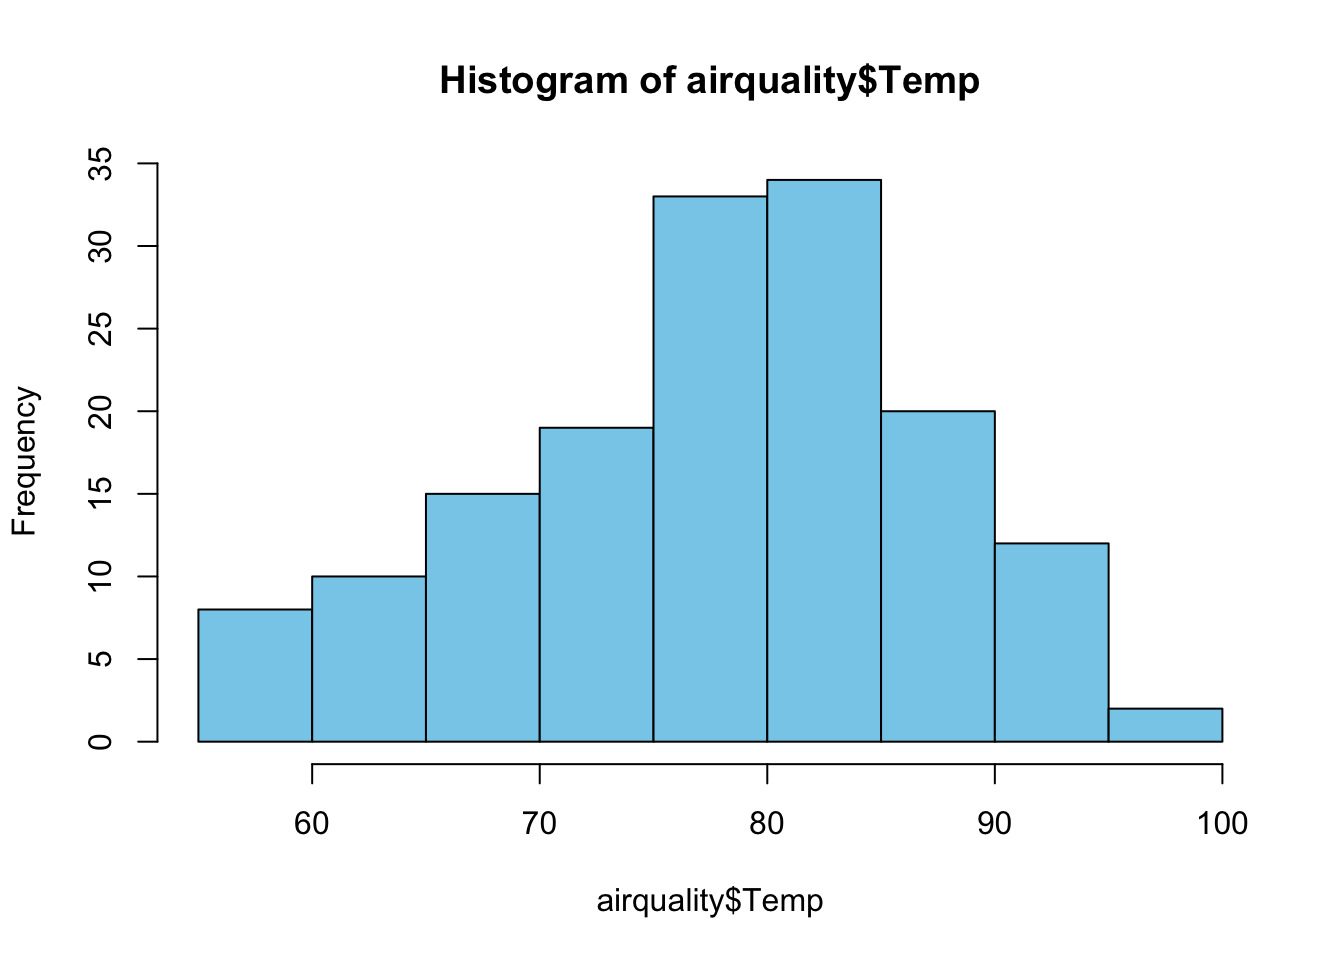
\includegraphics{Chocolate_files/figure-latex/unnamed-chunk-4-1.pdf}

According to the boxplot above it would appear that Australia's median
chocolate rating is superior to the other countries with the U.K.
falling in dead last. The table below provides a 5 number summary to
solidify and further compare the values shown in the boxplot.

\begin{Shaded}
\begin{Highlighting}[]
\NormalTok{choc1 }\OperatorTok\StringTok{ }
\StringTok{  }\KeywordTok{group_by}\NormalTok{(Location) }\OperatorTok\StringTok{ }
\StringTok{  }\KeywordTok{summarize}\NormalTok{(}\DataTypeTok{Min =} \KeywordTok{min}\NormalTok{(Rating),}
            \DataTypeTok{Q1 =} \KeywordTok{quantile}\NormalTok{(Rating, }\FloatTok{0.25}\NormalTok{),}
            \DataTypeTok{Median =} \KeywordTok{median}\NormalTok{(Rating),}
            \DataTypeTok{Q3 =} \KeywordTok{quantile}\NormalTok{(Rating, }\FloatTok{0.75}\NormalTok{),}
            \DataTypeTok{Max =} \KeywordTok{max}\NormalTok{(Rating),}
            \DataTypeTok{Mean =} \KeywordTok{mean}\NormalTok{(Rating),}
            \DataTypeTok{sd =} \KeywordTok{sd}\NormalTok{(Rating),}
            \StringTok{"# of Companies"}\NormalTok{ =}\StringTok{ }\KeywordTok{n}\NormalTok{()) }\OperatorTok\StringTok{ }
\StringTok{  }\KeywordTok{pander}\NormalTok{()}
\end{Highlighting}
\end{Shaded}

\begin{longtable}[]{@{}ccccccccc@{}}
\toprule
\begin{minipage}[b]{0.13\columnwidth}\centering
Location\strut
\end{minipage} & \begin{minipage}[b]{0.06\columnwidth}\centering
Min\strut
\end{minipage} & \begin{minipage}[b]{0.06\columnwidth}\centering
Q1\strut
\end{minipage} & \begin{minipage}[b]{0.08\columnwidth}\centering
Median\strut
\end{minipage} & \begin{minipage}[b]{0.06\columnwidth}\centering
Q3\strut
\end{minipage} & \begin{minipage}[b]{0.05\columnwidth}\centering
Max\strut
\end{minipage} & \begin{minipage}[b]{0.07\columnwidth}\centering
Mean\strut
\end{minipage} & \begin{minipage}[b]{0.08\columnwidth}\centering
sd\strut
\end{minipage} & \begin{minipage}[b]{0.15\columnwidth}\centering
\# of Companies\strut
\end{minipage}\tabularnewline
\midrule
\endhead
\begin{minipage}[t]{0.13\columnwidth}\centering
Australia\strut
\end{minipage} & \begin{minipage}[t]{0.06\columnwidth}\centering
2.5\strut
\end{minipage} & \begin{minipage}[t]{0.06\columnwidth}\centering
3\strut
\end{minipage} & \begin{minipage}[t]{0.08\columnwidth}\centering
3.5\strut
\end{minipage} & \begin{minipage}[t]{0.06\columnwidth}\centering
3.75\strut
\end{minipage} & \begin{minipage}[t]{0.05\columnwidth}\centering
4\strut
\end{minipage} & \begin{minipage}[t]{0.07\columnwidth}\centering
3.357\strut
\end{minipage} & \begin{minipage}[t]{0.08\columnwidth}\centering
0.4177\strut
\end{minipage} & \begin{minipage}[t]{0.15\columnwidth}\centering
49\strut
\end{minipage}\tabularnewline
\begin{minipage}[t]{0.13\columnwidth}\centering
Germany\strut
\end{minipage} & \begin{minipage}[t]{0.06\columnwidth}\centering
1.5\strut
\end{minipage} & \begin{minipage}[t]{0.06\columnwidth}\centering
3\strut
\end{minipage} & \begin{minipage}[t]{0.08\columnwidth}\centering
3.25\strut
\end{minipage} & \begin{minipage}[t]{0.06\columnwidth}\centering
3.5\strut
\end{minipage} & \begin{minipage}[t]{0.05\columnwidth}\centering
4\strut
\end{minipage} & \begin{minipage}[t]{0.07\columnwidth}\centering
3.179\strut
\end{minipage} & \begin{minipage}[t]{0.08\columnwidth}\centering
0.4758\strut
\end{minipage} & \begin{minipage}[t]{0.15\columnwidth}\centering
35\strut
\end{minipage}\tabularnewline
\begin{minipage}[t]{0.13\columnwidth}\centering
Switzerland\strut
\end{minipage} & \begin{minipage}[t]{0.06\columnwidth}\centering
2\strut
\end{minipage} & \begin{minipage}[t]{0.06\columnwidth}\centering
3\strut
\end{minipage} & \begin{minipage}[t]{0.08\columnwidth}\centering
3.25\strut
\end{minipage} & \begin{minipage}[t]{0.06\columnwidth}\centering
3.75\strut
\end{minipage} & \begin{minipage}[t]{0.05\columnwidth}\centering
4\strut
\end{minipage} & \begin{minipage}[t]{0.07\columnwidth}\centering
3.342\strut
\end{minipage} & \begin{minipage}[t]{0.08\columnwidth}\centering
0.4665\strut
\end{minipage} & \begin{minipage}[t]{0.15\columnwidth}\centering
38\strut
\end{minipage}\tabularnewline
\begin{minipage}[t]{0.13\columnwidth}\centering
U.K.\strut
\end{minipage} & \begin{minipage}[t]{0.06\columnwidth}\centering
1.75\strut
\end{minipage} & \begin{minipage}[t]{0.06\columnwidth}\centering
2.75\strut
\end{minipage} & \begin{minipage}[t]{0.08\columnwidth}\centering
3\strut
\end{minipage} & \begin{minipage}[t]{0.06\columnwidth}\centering
3.5\strut
\end{minipage} & \begin{minipage}[t]{0.05\columnwidth}\centering
4\strut
\end{minipage} & \begin{minipage}[t]{0.07\columnwidth}\centering
3.055\strut
\end{minipage} & \begin{minipage}[t]{0.08\columnwidth}\centering
0.4936\strut
\end{minipage} & \begin{minipage}[t]{0.15\columnwidth}\centering
96\strut
\end{minipage}\tabularnewline
\bottomrule
\end{longtable}

Since the data appears to be slightly skewed in several of the groups,
we'll now compare the countries using the Kruskal-Wallis Rank Sum Test.
Our Null and alternative hypthosis are thus:

\[
  H_0: \text{All samples represent a sample of data from the same distribution.}
\] \[
  H_a: \text{At least one distribution is stochastically different than the others.}
\]

Our level of Significance will be:

\[
alpha = 0.05
\]

Performing the Kruskal-Wallis Rank Sum test we get the following
results.

\begin{Shaded}
\begin{Highlighting}[]
\KeywordTok{kruskal.test}\NormalTok{(Rating }\OperatorTok{~}\StringTok{ }\NormalTok{Location, }\DataTypeTok{data =}\NormalTok{ choc1)}
\end{Highlighting}
\end{Shaded}

\begin{verbatim}

    Kruskal-Wallis rank sum test

data:  Rating by Location
Kruskal-Wallis chi-squared = 17.471, df = 3, p-value = 0.0005655
\end{verbatim}


\end{document}
